\documentclass[11pt]{standalone}
\usepackage[outline]{contour}
\contourlength{2.1pt}
\usepackage{pgfplots}
\usetikzlibrary{hobby}
\pgfplotsset{compat=newest}

\begin{document}
	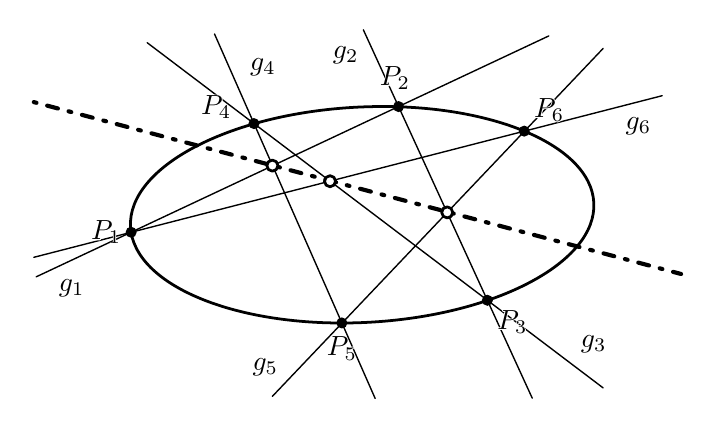
\begin{tikzpicture}[line cap=round, line join=round, line width=0.5, x=0.6cm, y=0.6cm]
	\clip(0.07,-5.24) rectangle (14.04,2.69);
	\draw [line width=1, rotate around={-177.03:(7.15,-1.27)}] (7.15,-1.27) ellipse (4.91 and 2.28);
	\draw [domain=0.2:13.5] plot(\x,{(-18.49--2.14*\x)/8.32});
	\draw [domain=2.6:12.25] plot(\x,{(-21.44--3.74*\x)/-4.94});
	\draw [domain=5.25:12.25] plot(\x,{(--41.05-4.06*\x)/-3.86});
	\draw [domain=0.25:11.1] plot(\x,{(--15.29-2.66*\x)/-5.66});
	\draw [domain=7.175:10.75] plot(\x,{(--34.39-4.1*\x)/1.88});
	\draw [domain=4.025:7.425] plot(\x,{(--21.74-4.22*\x)/1.86});
	\draw [line width=1.5,dash pattern=on 1pt off 4pt on 4pt off 4pt,domain=0.2:13.9] plot(\x,{(-4.31--0.98*\x)/-3.69});
	\fill [color=black] (2.26,-1.64) circle (2pt) node[left] {\contour{white}{$P_1$}};
	\fill [color=black] (7.92,1.02) circle (2pt) node[shift={(-0.075,0.6)}] {\contour{white}{$P_2$}};
	\fill [color=black] (9.8,-3.08) circle (2pt) node[below right] {\contour{white}{$P_3$}};
	\fill [color=black] (4.86,0.66) circle (2pt) node[shift={(-0.8,0.35)}] {\contour{white}{$P_4$}};
	\fill [color=black] (6.72,-3.56) circle (2pt) node[below=1.5] {\contour{white}{$P_5$}};
	\fill [color=black] (10.58,0.5) circle (2pt) node[above right] {\contour{white}{$P_6$}};
	\draw[color=black] (13,0.6) node {$g_6$};
	\draw[color=black] (12.05,-4) node {$g_3$};
	\draw[color=black] (5.1,-4.5) node {$g_5$};
	\draw[color=black] (1,-2.825) node {$g_1$};
	\draw[color=black] (6.8,2.1) node {$g_2$};
	\draw[color=black] (5.05,1.85) node {$g_4$};
	\draw [line width=1,fill=white] (8.95,-1.22) circle (2pt);
	\draw [line width=1,fill=white] (5.25,-0.23) circle (2pt);
	\draw [line width=1,fill=white] (6.47,-0.56) circle (2pt);
	\end{tikzpicture}
\end{document}